\documentclass[border=10pt]{standalone}

\usepackage{tikz}
\usepackage{tikzsymbols}
\usetikzlibrary{calc,patterns,shapes.geometric}

\def\centerarc[#1](#2)(#3:#4:#5){\draw[#1] ($(#2)+({#5*cos(#3)},{#5*sin(#3)})$) arc (#3:#4:#5);}

\begin{document}
	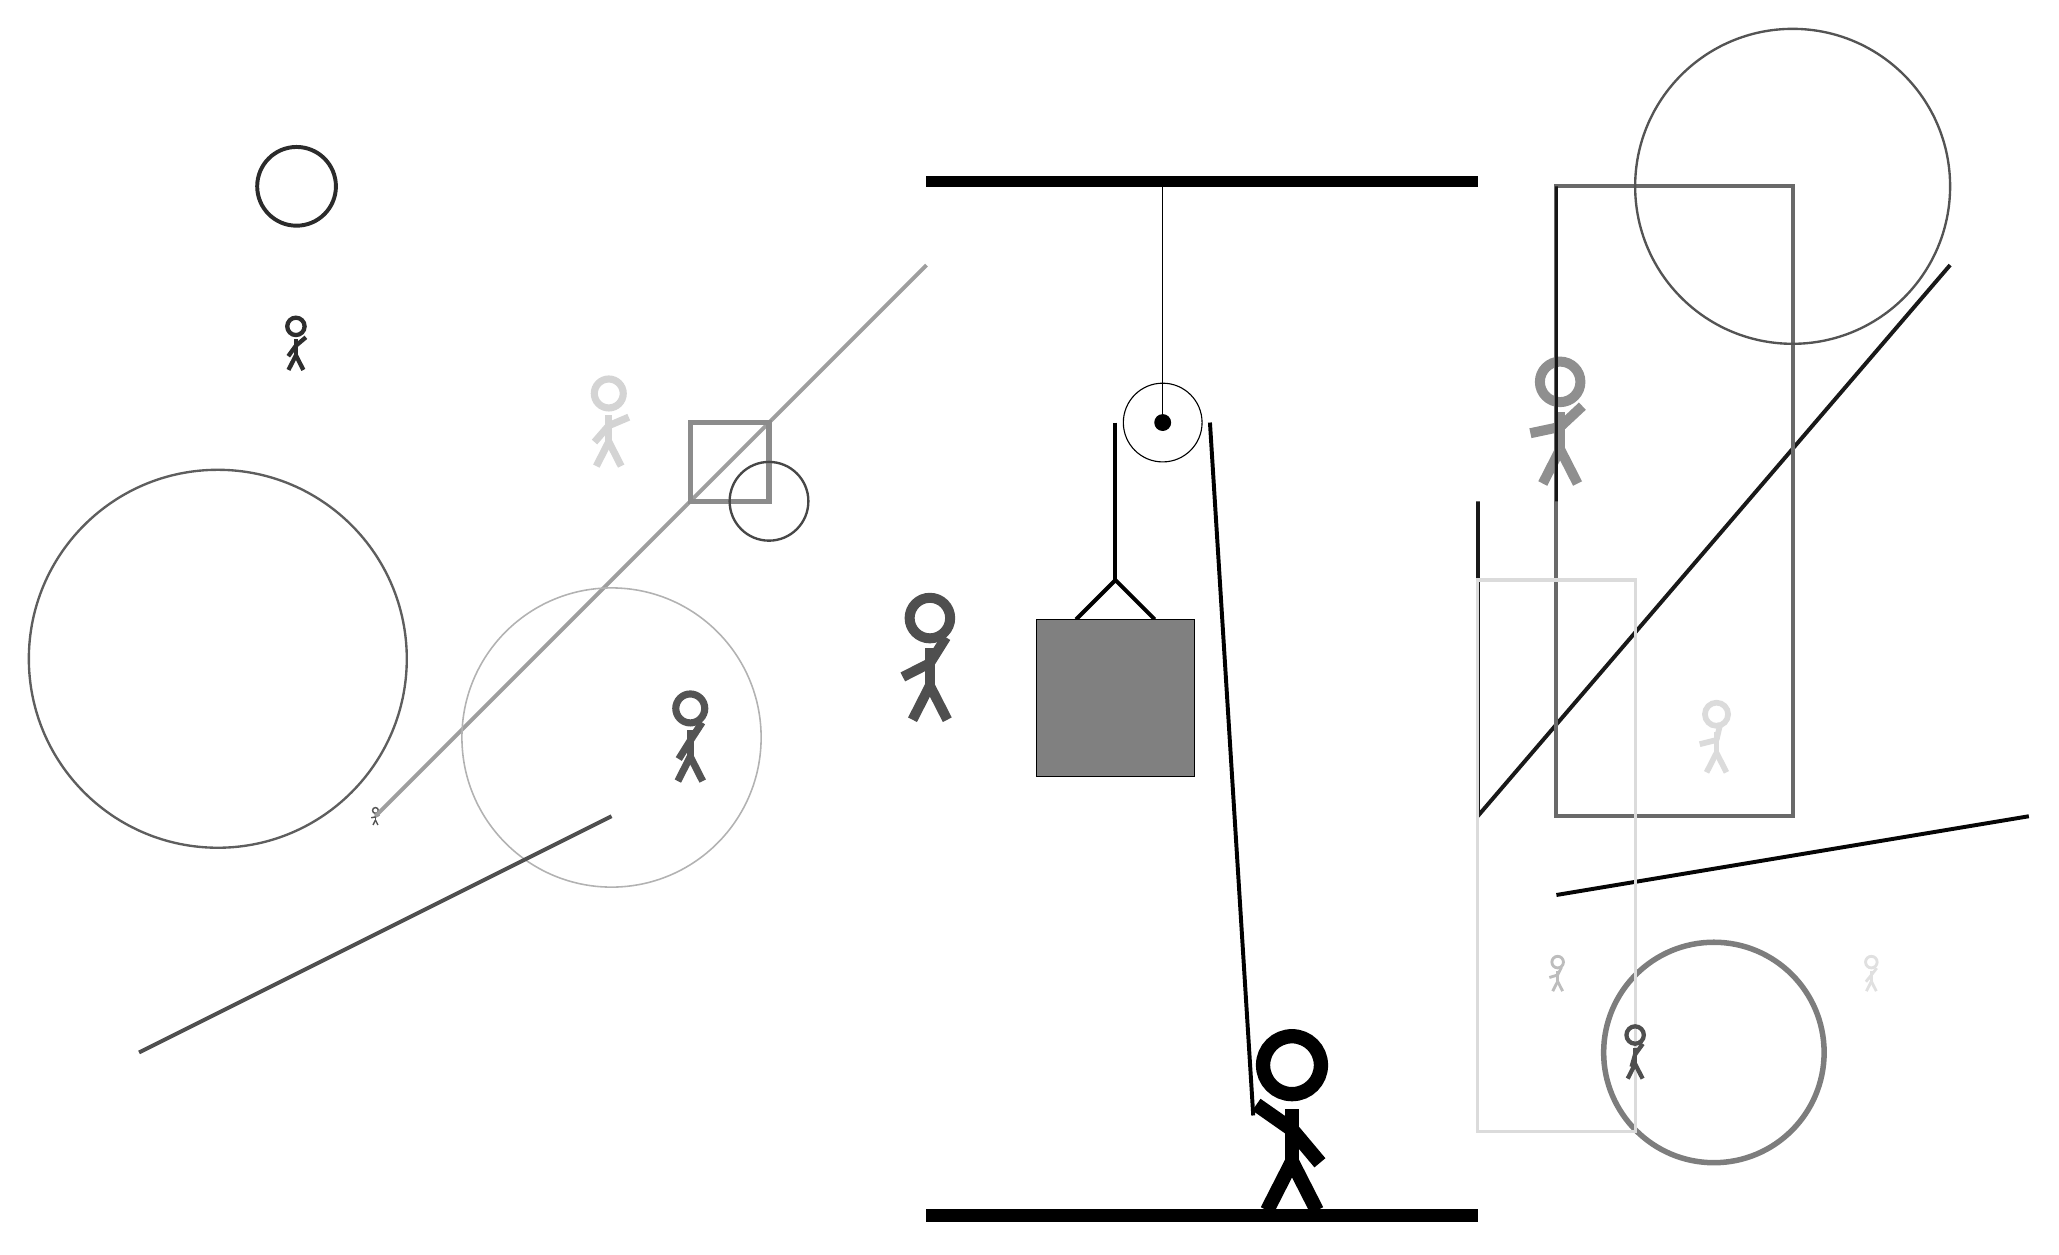
\begin{tikzpicture}
		%%%%% START %%%%%
		
		\draw[fill=black] (-2, 10) rectangle (5, 10.125);
		
		\draw[line width=0.5mm, color=black!90](5, 2) -- (11, 9);
		
		\node[line width=0.7mm, color=black!12] at (10, 0) {\Strichmaxerl[2][51][52]};
		\node[line width=0.2mm, color=black!67] at (-9, 2) {\Strichmaxerl[1][12][24]};
		\draw[line width=0.5mm, color=black!38](-2, 9) -- (-9, 2);
		\draw[line width=0.7mm, color=black!45] (-4, 7) rectangle (-5, 6);
		\draw [line width=0.2mm, color=black!30](-6, 3) circle (1.9);
		\draw [line width=0.3mm, color=black!63](-11, 4) circle (2.4);
		\draw [line width=0.3mm, color=black!72](-4, 6) circle (0.5);
		\draw[line width=0.5mm, color=black!69](-6, 2) -- (-12, -1);
		\node[line width=0.6mm, color=black!44] at (6, 7) {\Strichmaxerl[7][12][43]};
		
		\draw[line width=0.5mm, color=black!90] (5, 6) rectangle (5, 2);
		\node[line width=0.6mm, color=black!17] at (-6, 7) {\Strichmaxerl[5][49][23]};
		\node[line width=0.3mm, color=black!14] at (8, 3) {\Strichmaxerl[4][14][77]};
		
		\draw[line width=0.5mm, color=black!98](6, 1) -- (12, 2);
		\node[line width=0.7mm, color=black!69] at (-2, 4) {\Strichmaxerl[7][27][58]};
		\draw [line width=0.7mm, color=black!51](8, -1) circle (1.4);
		
		\draw[line width=0.5mm, color=black!59] (6, 10) rectangle (9, 2);
		\draw[line width=0.4mm, color=black!14] (7, -2) rectangle (5, 5);
		\draw [line width=0.5mm, color=black!83](-10, 10) circle (0.5);
		\node[line width=0.2mm, color=black!69] at (7, -1) {\Strichmaxerl[3][74][54]};
		\draw[line width=0.4mm, color=black!91] (6, 6) rectangle (6, 10);
		
		\node[line width=0.3mm, color=black!26] at (6, 0) {\Strichmaxerl[2][17][64]};
		\node[line width=0.5mm, color=black!82] at (-10, 8) {\Strichmaxerl[3][54][40]};
		\draw [line width=0.3mm, color=black!67](9, 10) circle (2.0);
		\node[line width=0.5mm, color=black!67] at (-5, 3) {\Strichmaxerl[5][58][57]};
		
		
		\draw (1, 7) circle (0.5);
		\draw[fill=black] (1, 7) circle (0.1);
		\draw (1, 10) -- (1, 7);
		
		\draw[line width=0.5mm] (-0.1, 4.5) -- (0.4, 5.0) -- (0.9, 4.5);
		\draw[fill=black!50] (-0.6, 4.5) rectangle (1.4, 2.5);
		
		\draw[line width=0.5mm] (0.4, 7) -- (0.4, 5.0);
		\centerarc[line width=0.5mm](1, 7)(0:180:0.6);
		\draw[line width=0.5mm](1.6, 7) -- (2.15, -1.8);
		
		\node at (2.6, -1.9) {\Strichmaxerl[10][-35][-50]};
		
		\draw[fill=black] (-2, -3) rectangle (5, -3.15);
		
		%%%%% END %%%%%
	\end{tikzpicture}
\end{document}